% !TEX root = arbeit.tex
% Damit Latex weiss, wo die main Datei ist.
\section{Introduction}
	
	\subsection{Mission Introduction} % Search for a better title
	% Rockets:
	% https://www.grc.nasa.gov/www/k-12/TRC/Rockets/history_of_rockets.html
	
	Investigation of the stars and the night sky started a long time ago. The back then, the movement of the Sun, the Moon and the stars was used to derive time, for navigation and for religious rituals. First records of systematic observations of the night sky date back to the Assyro-Babylonians around 1000 BCE. In the third century BCE Greek astronomers tried to estimate the distances between the different cosmic objects with geometrical tools \cite{space_history}. The invention of telescopes in the early 17th century allowed then a closer look at the objects in the night sky and lead to the discovery of the Galilean moons' Io, Europa, Callisto and Ganymede by Galileo Galilei in 1610. Galileo discovered that these objects were orbiting around another object than the Sun (Jupiter).
	\begin{wrapfigure}{r}{0.5\textwidth}
		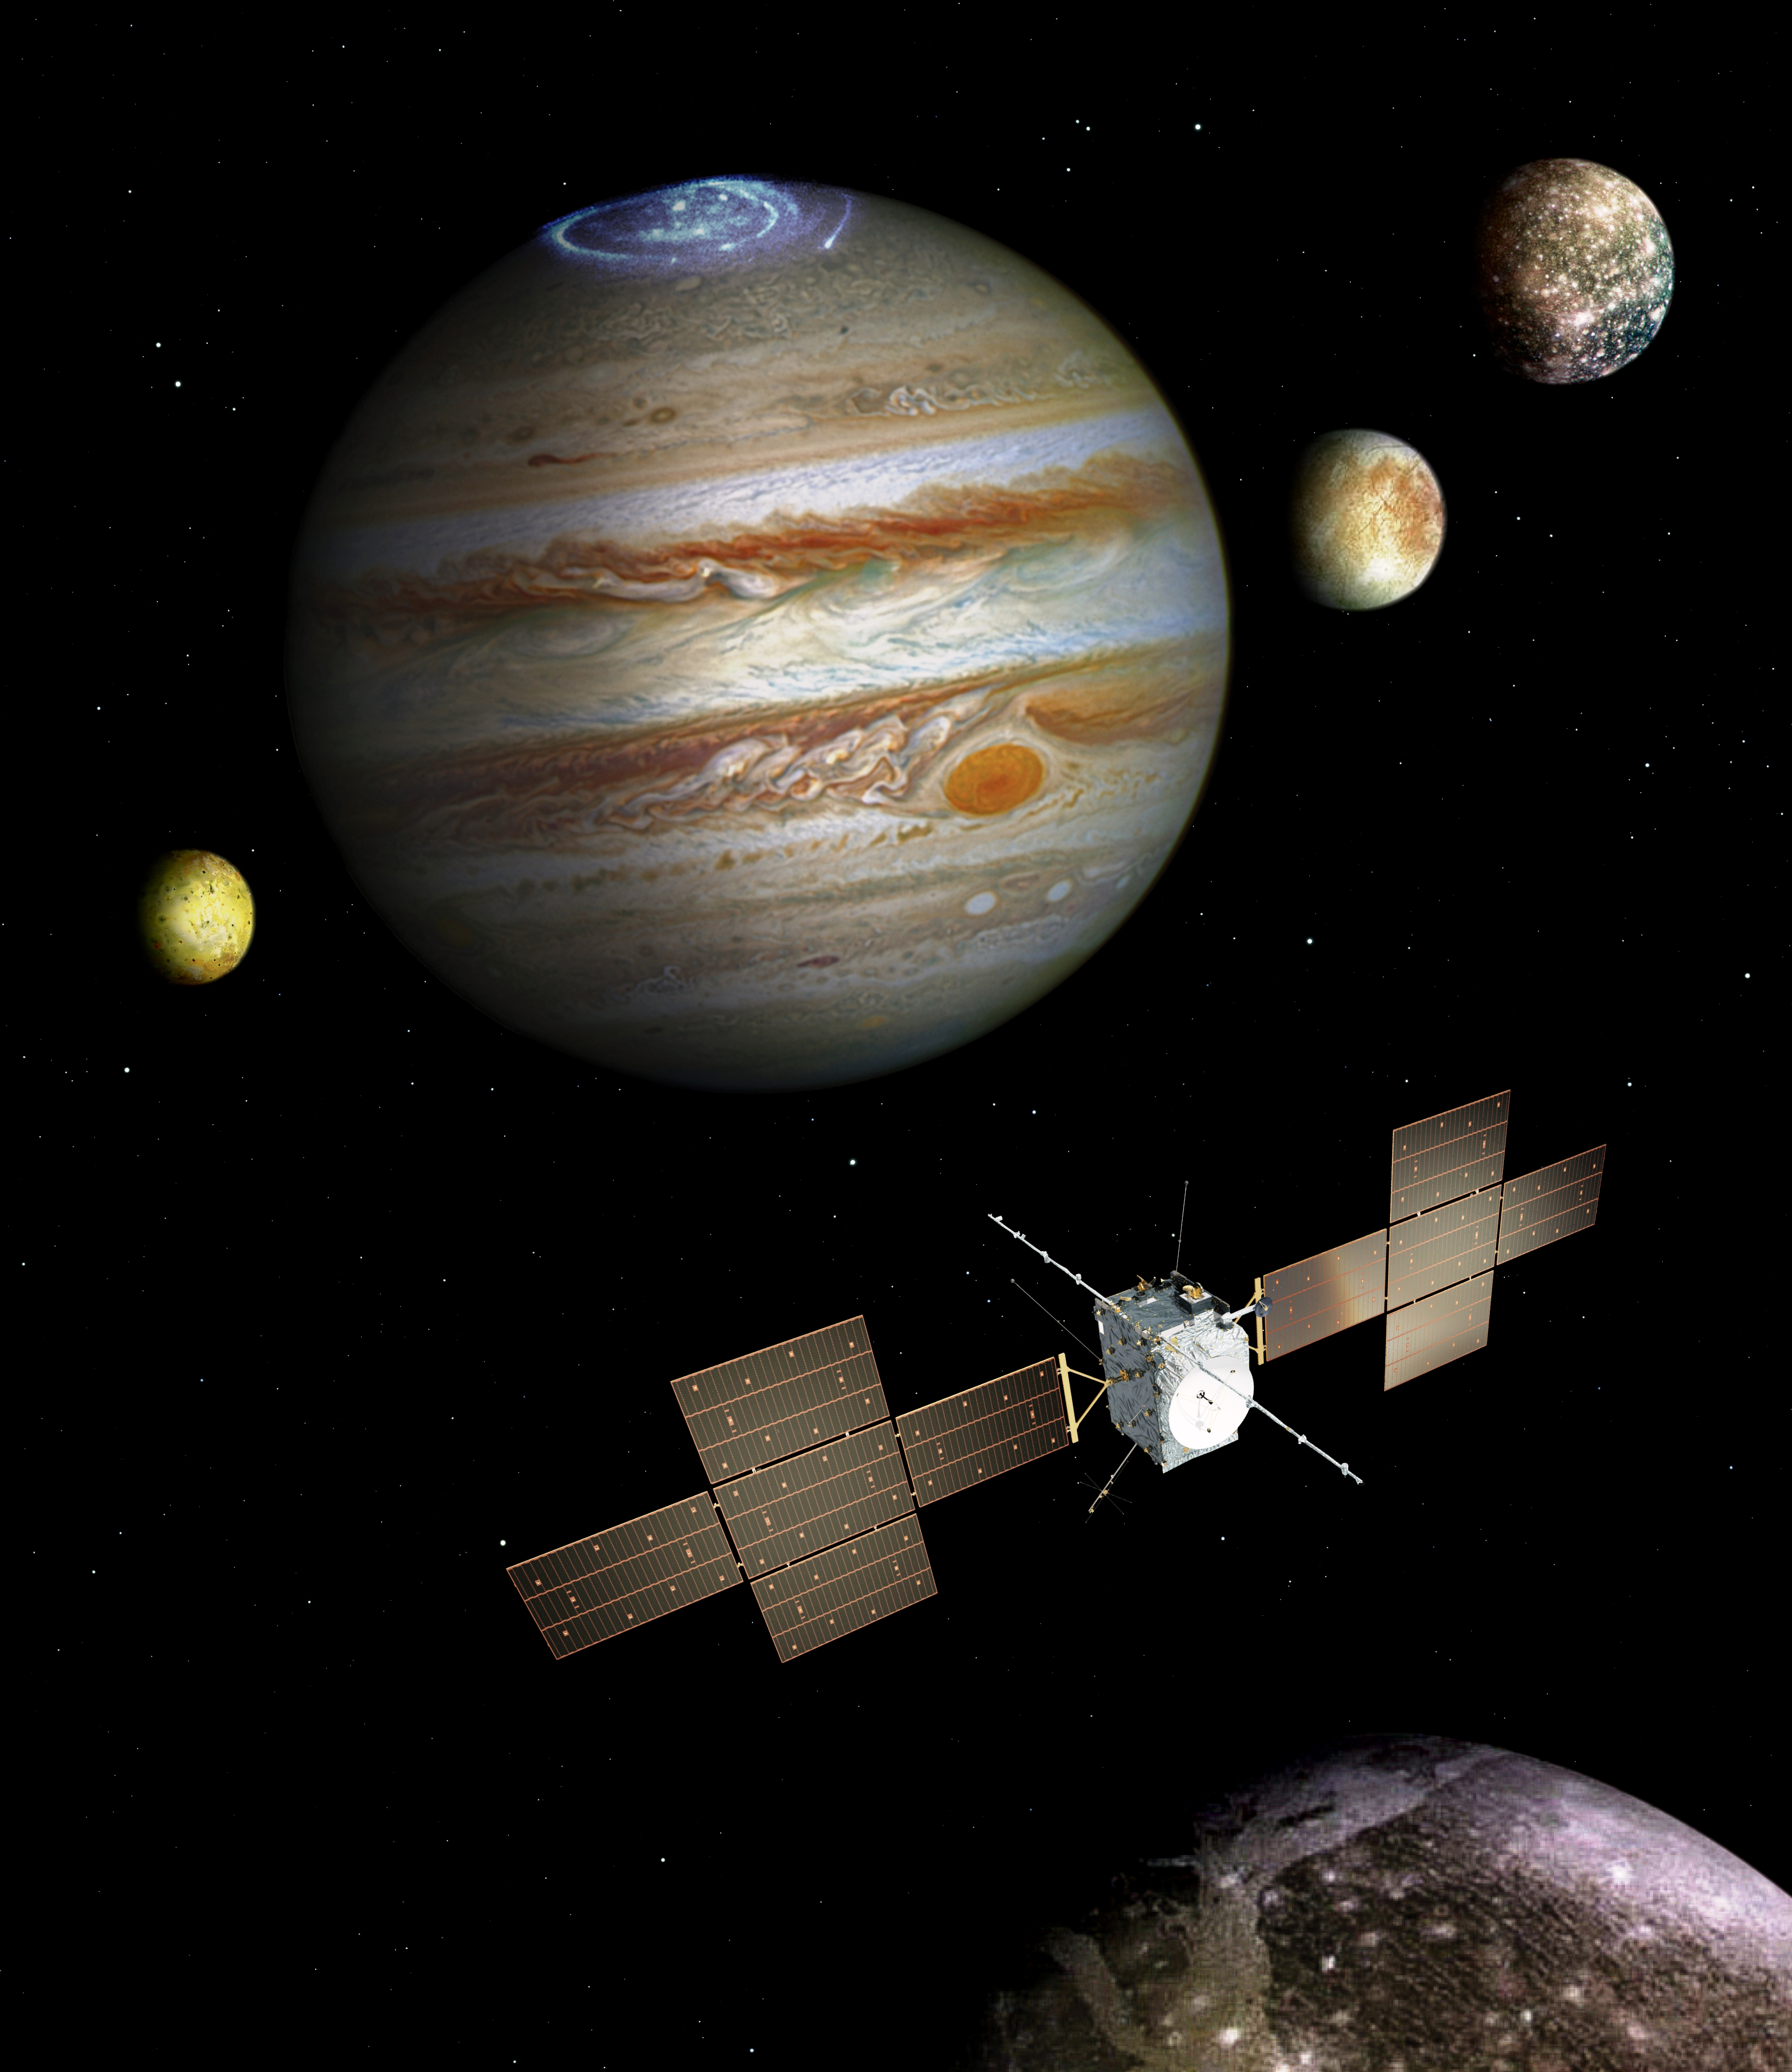
\includegraphics[width=\linewidth]{Bilder/Juice_mission.jpg}
		\caption{Artist impression of the Juice mission exploring the Jupiter system \cite{JUICE_Pic}.}
		\label{fig:JUICE}
	\end{wrapfigure}
	The invention of the first modern rockets during the cold war, opened the opportunity of on site exploration of solar system bodies. The data acquired through those in situ measurements gave further insight into the formation processes and history of our solar system. The missions Pioneer 10~\&~11 and Voyager 1~\&~2 were the first space missions, which took close images of Jupiter and its icy moons. They discovered Jupiter's ring system and detected more small moons of Jupiter than only the four big Galilean moons. The missions Galileo (1995-2003) and JUNO (2016-2025) were two missions specifically with the objective to further investigate Jupiter itself (JUNO) and its icy moons (Galileo) with the main outcome of giving strong evidence for salty subsurface oceans on the moons Europa, Ganymede and Callisto by measuring the induced magnetic fields. These oceans could be environments where life might be possible. In addition, Galileo observed that Ganymede has an intrinsic magnetic field interacting with the strong magnetic field of Jupiter \cite{Jupiter_SpaceMission}.\\
	The JUpiter ICy moons Explorer JUICE built by the European Space Agency ESA has the objective to further investigate Jupiter, its environment and its icy moons with regards to their potential of harbouring life. JUICE will characterise Jupiter as a planet, Jupiter's plasma environment and it will characterise Jupiter's icy moons Europa, Ganymede and Callisto. JUICE will characterise Jupiter's atmospheric dynamics, composition and chemistry and the atmosphere's vertical structure. It will characterise Jupiter's magnetosphere to understand the role of the moons as sources and sinks for the magnetospheric plasma. JUICE will study Jupiter's ring system, its small satellites and it will study Io's activity and surface composition with its remote sensing instruments.\\
	With regards to the icy moons, the main objectives are to characterise their potential subsurface oceans and their non-icy material. Europa consists mainly out of silicates with a water layer and an ice crust on top of that. Europa's surface is fairly young showing almost no impact craters which implies that the icy layer frequently moves similar to plate tectonics. Ganymede is until now the only satellite in our solar system known having an intrinsic magnetic field generated by a magnetic dipole field. Therefore, JUICE will investigate the interaction processes of that magnetic field with Jupiter's magnetic field because it is strong enough to successfully shield the moon against the plasma flow from Jupiter's magnetosphere. Callisto is the outer most of the Galilean moons and by far the most cratered. It lacks of small craters indicating some minor erosion processes. Compared to the other three Galilean moons, Callisto lacks any greater tectonic activity \cite{red_book}.\\
	\begin{figure}[h]
		\centering
		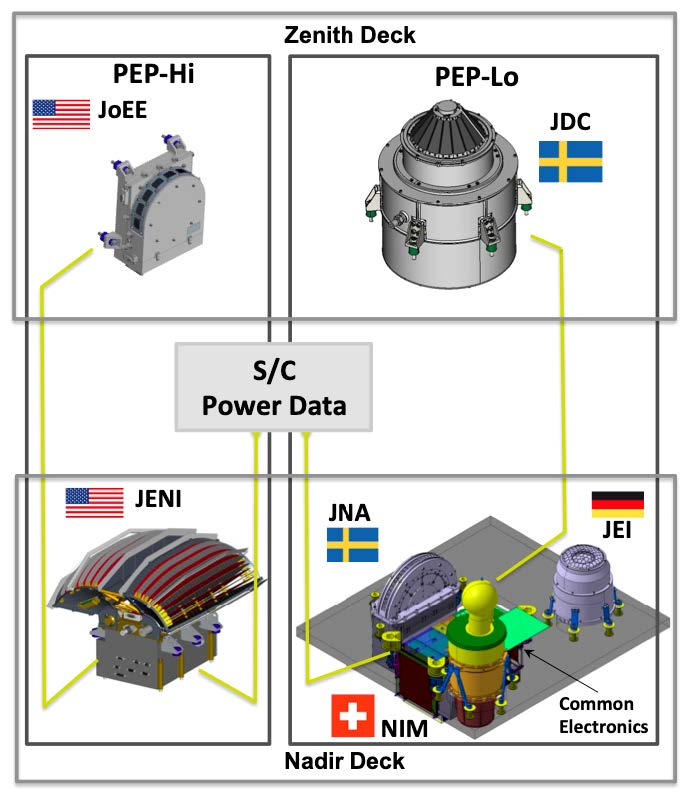
\includegraphics[width=.7\textwidth]{Bilder/PEP_Instruments.jpg}
		\caption{Sketch of the six PEP instruments \cite{PEP_inst}.}
		\label{fig:PEPInst}
	\end{figure}
	To fulfil the scientific goals, JUICE has an instrument suit consisting of 11 instruments on board ranging from cameras to magneto and gravity meters to particle detectors. One of these instruments is the Particle and Environment Package System PEP (Fig.~\ref{fig:PEPInst}). The main focus of PEP is to characterise Jupiter's plasma environment and the composition of the icy moons' exosphere. Therefore, PEP has six sensors to measure neutral particles, ions and electrons with energies from thermal ($<$~5~eV) up to 5~MeV (ions) \cite{PEP_inst}. One of these six sensors is the Neutral Gas and Ion Mass Spectrometer NIM. The focus of NIM lays on the characterisation of the icy moons exosphere and the detection of ions with an energy less than 100~eV to complete the plasma measurements for slow ions of the other PEP instruments. With the capability of measuring slow ions, NIM is able to detect a potential ionosphere of the icy moons \cite{Diss_Meyer}. NIM will be the first mass spectrometer taking in situ measurements of the icy moons exosphere. The exosphere is formed by particles released from the moons' surface by ion bombardment, sublimation and photon interaction processes. By sampling the exosphere, we get a deeper insight in the surface composition and the formation processes involved of the icy moons themself. For example, there are two major theories about when the icy moons were formed. One suggests that the icy moons' were formed in the protostar nebula of our solar system implying that the moons have a similar age as Jupiter. Another hypothesis suggests that the icy moons' were formed in the subnebula of Jupiter, implying that they are younger than Jupiter. By determining the particle density and isotope ratios of the detected species, we can distinguish between these two formation processes giving us a deeper insight in how our solar system was formed and which processes in the formation of the icy moons' are the most relevant \cite[and references therein]{Vorburger2015}.\\
	
	The instruments sent to space missions are customised to fulfil the specific requirements. For space missions, the instruments have to be small, light and low power consumptive. Especially for missions having targets in the outer solar system, such as JUICE with target Jupiter, power is a very limited resource. At Jupiter, the solar flux density is by a factor 25 lower than at Earth because Jupiter is five times farther away from the Sun than Earth. Therefore, missions flying to the outer solar system often use radioisotope thermoelectric generators (RTGs) as power sources instead of solar panels because they are longer lasting and provide more power. The biggest drawback is that they are very inefficient and produce a lot of heat, which cannot be used \cite{Power_Space}. Another main challenge is the harsh radiation environment of Jupiter. The penetrating particles lead to upset in the electronics and damage components. Therefore, a proper shielding concept was necessary.\\

	NIM is a time-of-flight mass spectrometer with heritage from previous TOF instruments developed at the university of Bern. These are the RTOF/ROSINA/Rosetta \cite{Balsiger2007a,Scherer2006}, P-BACE/ MEAP \cite{Abplanalp2009a} and NGMS/Luna-Resurs \cite{Wurz2012264,Fausch_IEEE}. Mass spectrometers are single ion counting instruments. Therefore, they can estimate the density distributions of the measured species much more precisely than remote sensing instruments. The biggest advantages of time-of-flight mass spectrometers compared to other mass spectrometer types is that they are extremely robust from the mechanical point of view and have a better sensitivity than scanning instruments. Magnetic sectors are heavy and require high accuracy mechanics. Quadrupole mass spectrometers fulfil the requirements regarding size, weight and power but have a lower sensitivity than TOF instruments because to increase the mass resolution they loose sensitivity \cite{Quadrupol_WorkPrinc}. In addition, scanning instruments have a relatively long cadence \cite{MassSpec_Overview} leading to a bad spacial resolution during the flybys of the spacecraft on the icy moons. Therefore, TOF instruments are often used in space missions.\\
	NIM is designed to measure complex molecules up to 1000~u with a mass resolution up to $m/\Delta m$ 1000 with a signal-to-noise ratio (SNR) of 6 decades. In the icy moons exosphere we only expect species with masses up to 100~u but with the ability to measure also species with higher masses, NIM is able to detect also potential organic compounds if they are present \cite{NIM_Req_dMSNR}. To separate species with such high masses, it requires a mass resolution of $m/\Delta m$ 1000 to be able to distinguish between the different unit masses. With a SNR of 6 decades, NIM is able to measure down to partial pressures of 10\textsuperscript{-16}~mbar corresponding to a particle density of 1~cm\textsuperscript{-3}. During the flybys at the icy moons, the spacecraft velocity is 1-8~km/s. Depending on the mass of the particles, the highest energy they have is up to 100~eV which is the highest energy NIM has to deal with. NIM is designed to measure particles with thermal energy up to energies of 100~eV. NIM has an open and a closed source entrance for neutral particles and ions. Through the open source entrance slit, neutral particles and ions enter the ionisation region directly without interacting with the instrument structure. The closed source consists of an antechamber which thermalises incoming neutrals. Neutrals with higher speeds are therefore easier to detect than with the open source channel where particles enter the ionisation region with spacecraft velocity. As mentioned above, mass and power are for these missions very limited resources. The NIM ion-optical system has a mass of 3.13~kg from which 48~\% is shielding mass to shield the detector locally to reduce noise induced by high energetic particles originating from Jupiter's plasma environment. The power allocated for the NIM instrument from the spacecraft is 18.5~W.
	% (FoV, 10/3~pi), 10°x300°

	\subsection{Thesis Outline}
	This thesis follows up the PhD thesis of Stefan Meyer \cite{Diss_Meyer}. At the end of his thesis, the NIM prototype was built and the flight design the NIM was almost completed.\\	
	The objective of this thesis was to finalize the design of the NIM flight model, to build and test the NIM Proto-Flight-Model (PFM) to deliver it to the JUICE spacecraft and to build and test the NIM Flight-Spare (FS) model, which stays on Earth as a ground reference. This required environmental tests of various flight subcomponents as they came available with finally testing the ion-optical system of the NIM PFM and FS sensor. Ion-optical simulations were performed to set constrains on the design of the flight power supplies as they were still under development during the early phases of this thesis.\\
	The thesis consists of three main parts: Chap.~\ref{sec:theory} shows theoretical analyses of key components of the NIM instrument such as the performance of the closed source antechamber. In addition, it sums up the theoretical aspects needed to understand the performance results of the different subsystems presented in Chap.~\ref{sec:Exp}. Chap.~\ref{sec:setup} compares the design of the NIM prototype with the final flight design and shows the main differences between the two models. A special focus lays there in the improvements done on the design of the detector. Chap.~\ref{sec:Exp} sums up the performance tests of different subsystems partially tested stand alone (detector) or as part of the NIM Prototype (antechamber, ion-mirror). The chapter ends with performance tests of the two NIM flight models (PFM and FS).
	
	
	% Instruments on JUICE
	\begin{comment}
		\begin{itemize}
			\item Planetary Radio Interferometry and Doppler Experiment (PRIDE \cite{PRIDE_JUICE})
			\item Laser Altimeter (GALA (Ganymede Laser Altimeter) \cite{GALA_JUICE})
			\item Radio Science Experiment (3GM (Geodesy and Geophysics of Jupiter and the Galilean Moons 		\cite{3GM_JUICE}))
			\item Ice Penetrating Radar (RIME (Radar for Icy Moon Exploration)) % No Ref. found
			\item Visible-Infrared Hyperspectral Imaging Spectrometer (MAJIS (Moons And Jupiter Imaging Spectrometer 	\cite{MAJIS}))
			\item Ultraviolet Imaging Spectrograph (UVS) % no good Ref.
			\item Imaging System (JANUS (Jovis, Amorum ac Natorum Undique Scrutator \cite{JANUS})) 
			\item Magnetometer (J-MAG) % No Ref. found
			\item Submillimetre Wave Instrument (SWI) % Axel Murk
			\item Radio and Plasma Wave Instrument (RPWI \cite{RPWI_JUICE})
			\item Particle Package (PEP)
		\end{itemize}
	\end{comment}
	
	







